\documentclass[12pt]{article}

\usepackage[margin=1in]{geometry} % 1-inch margins
\usepackage{times}                % Times (Times New Roman–like) font
\usepackage{fancyhdr}             % For custom headers/footers
\usepackage{graphicx}             % For including images
\usepackage{titlesec}             % For section formatting
\usepackage{amsmath}              % For numbering control

\pagestyle{fancy}
\fancyhf{} % Clear default header and footer

% Header on the right side
\fancyhead[R]{Ultrasound Nerve Imaging And Clinical Decision Support System}

% Footer on the left side
\fancyfoot[L]{Pillai HOC College of Engineering \& Technology, Rasayani}
\fancyfoot[R]{\thepage}

% Horizontal lines in header & footer
\renewcommand{\headrulewidth}{0.4pt} 
\renewcommand{\footrulewidth}{0.4pt} 

% Enable figure numbering at section level (e.g., Figure 8.1, 8.2, 8.3)
\numberwithin{figure}{section}

\begin{document}

\setcounter{page}{51}

\vspace*{\fill}

\begin{center}
    {\Large \bf Chapter 8} \\[1em] % Line break with extra space (1em)
    {\Large \bf Result Analysis}
\end{center}
\vspace*{\fill}

\newpage

% SECTION 8: RESULT ANALYSIS
\setcounter{section}{8}

{\large \bf 8.1 Result Analysis}
\begin{figure}[h]

    {\small \bf 8.1.1 Front page of project} 
    \vspace{20pt}

    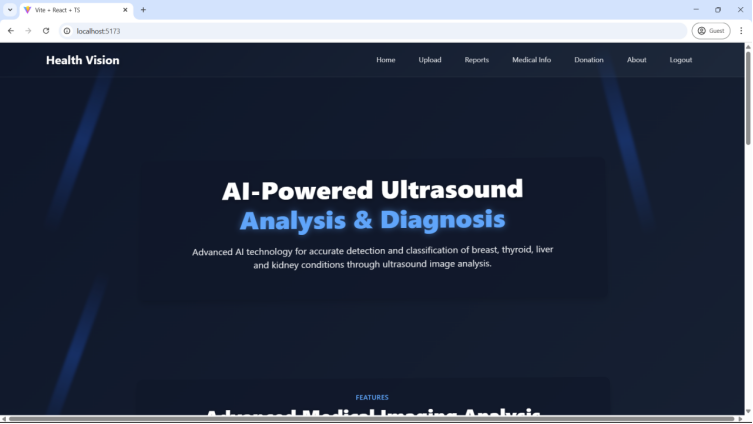
\includegraphics[width=0.9\textwidth]{41.png} % Replace with actual image
    \caption{Front page of project}
    \label{fig 8.1.1:dashboard_tab}
\end{figure}

\vspace{20pt}

In Figure 8.1.1 the image illustrates the homepage of a medical AI-based web platform named
”Health Vision”, which specializes in AI-powered ultrasound analysis and diagnosis. The webpage
highlights features such as advanced medical imaging analysis for detecting breast cancer, thyroid
disorders, kidney diseases, and other conditions using AI.

\newpage

\begin{figure}[h]

    {\Large \bf To Upload Ultrasound Images}
    \vspace{20pt}

    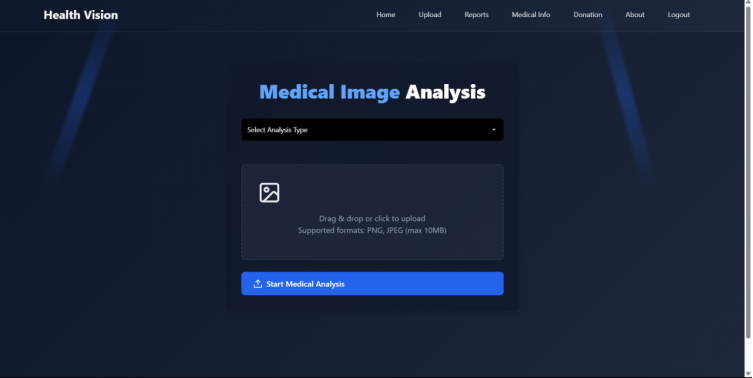
\includegraphics[width=0.9\textwidth]{42.png} 
    \caption{Upload Ultrasound Image}
    \label{fig:scan_tab}
\end{figure}

\vspace{20pt}

In Figure 8.2, we need to upload ultrasound images of the given diseases such as thyroid,
breast cancer, kidney stones, and liver disorders.

\newpage

\begin{figure}[h]

    {\Large \bf To Analyze Report Page }
    \vspace{20pt}

    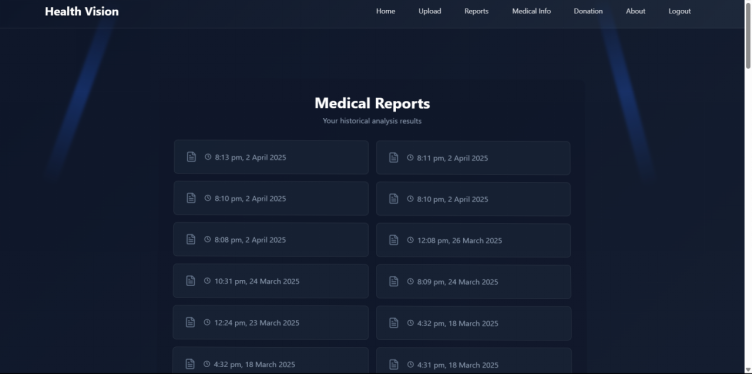
\includegraphics[width=0.9\textwidth]{43.png} 
    \caption{Report Page}
    \label{fig:selection_files}
\end{figure}

\vspace{20pt}

In Figure 8.3, the analysis report of the given ultrasound images is shown, and the user can view the report
anytime as it is stored in the database.

\newpage

\begin{figure}[h]

    {\Large \bf Medical Condition Videos For Thyroid}
    \vspace{10pt}

    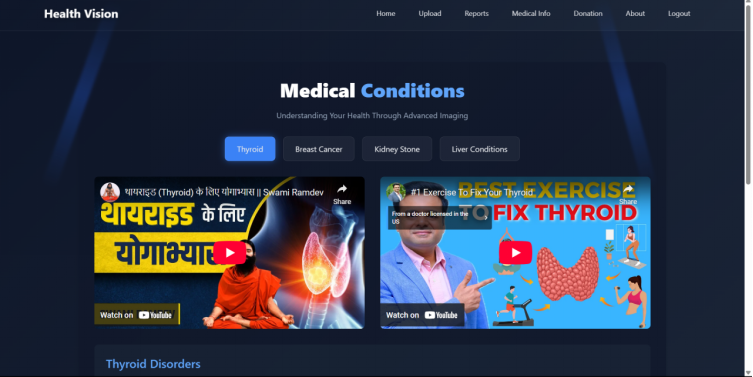
\includegraphics[width=0.9\textwidth]{44.png} 
    \caption{Thyroid Related Videos}
    \label{fig:reports}
\end{figure}

\vspace{20pt}

In Figure 8.4, recommended videos on thyroid disorders help users better understand the
disease. It provides YouTube videos that educate users on managing thyroid conditions through yoga, exercise, and lifestyle changes.

\newpage

\begin{figure}[h]

    {\Large \bf Medical Related Videos For Breast Cancer }
    \vspace{20pt}

    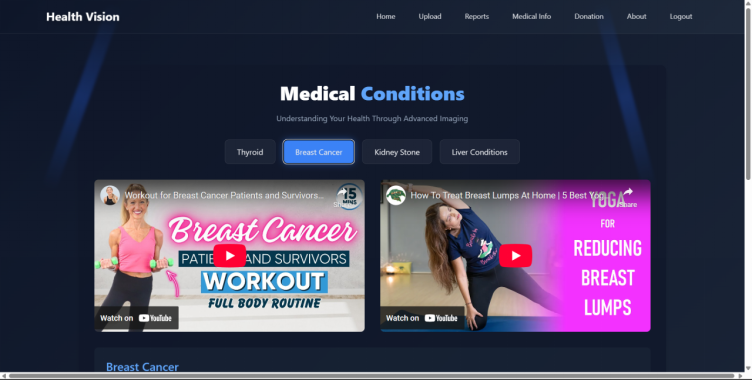
\includegraphics[width=0.9\textwidth]{45.png} 
    \caption{Breast Cancer related Videos}
    \label{fig:settings}
\end{figure}

\vspace{20pt}

In Figure 8.5, recommended videos about breast cancer help users better
understand the disease. These YouTube videos educate users on managing
breast cancer through yoga, exercise, and lifestyle changes.

\newpage

\begin{figure}[h]

    {\Large \bf Medical Related Videos For Kidney Stone}   
    \vspace{10pt}
    
    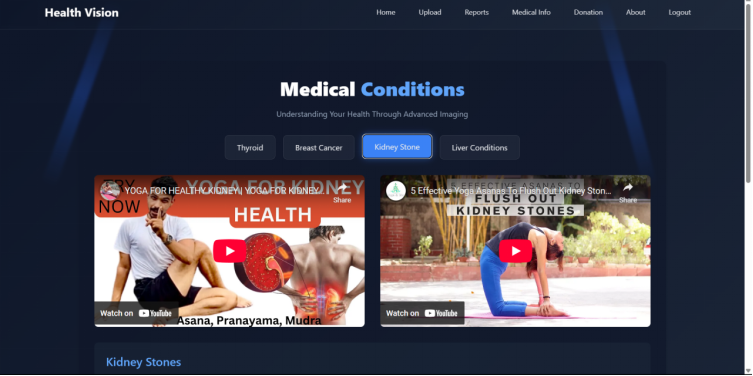
\includegraphics[width=0.8\textwidth]{46.png} 
    \caption{Kidney Stone Related Videos}
    \label{fig:complaint_tab}
\end{figure}

\vspace{20pt}

In Figure 8.6, recommended videos about kidney disorders help users better understand
the disease. These YouTube videos educate users on managing
kidney stones through yoga, exercise, and lifestyle changes.

\newpage

\begin{figure}[h]

    {\Large \bf Medical Related Videos For Liver}   
    \vspace{10pt}
    
    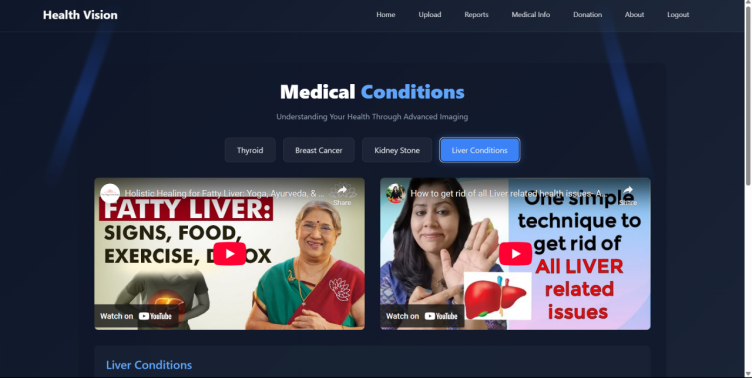
\includegraphics[width=0.8\textwidth]{47.png} 
    \caption{Liver Related Videos}
    \label{fig:complaint_tab}
\end{figure}

\vspace{20pt}

In Figure 8.7, recommended videos about liver disorders help users better
understand the disease. These YouTube videos educate users on managing
liver conditions through yoga, exercise, and lifestyle changes.

\newpage

\begin{figure}[h]

    {\Large \bf Donation Page}   
    \vspace{10pt}
    
    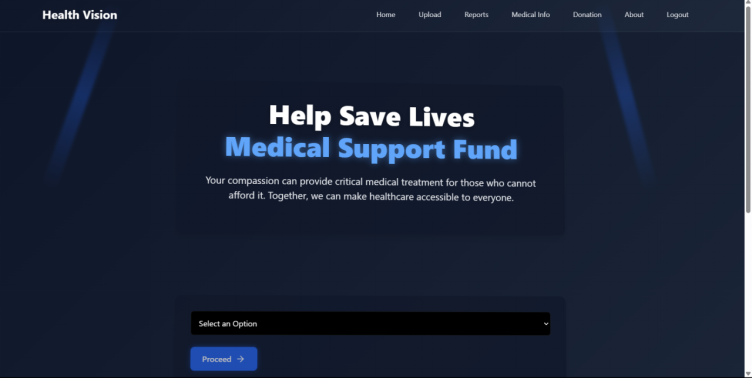
\includegraphics[width=0.8\textwidth]{48.png} 
    \caption{Donation Page}
    \label{fig:complaint_tab}
\end{figure}

\vspace{20pt}

In Figure 8.8, this page allows users to donate money or seek financial help if they
have any disease requiring financial assistance for treatment.

\end{document}
